\documentclass{standalone}
\usepackage{tikz}

\begin{document}

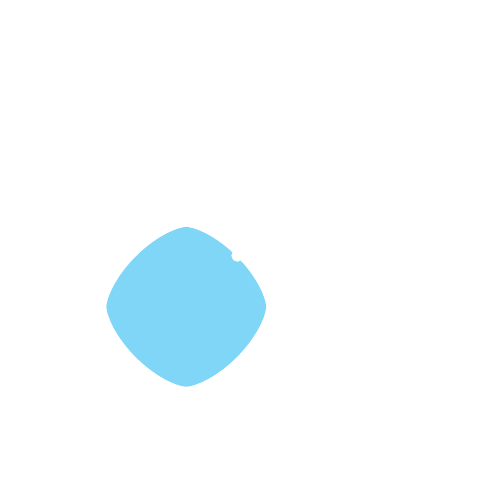
\begin{tikzpicture}

    % Axes
    \draw[->, thick, white] (-2,0) -- (3,0) node[right, text=white] {$\theta_1$};
    \draw[->, thick, white] (0,-2) -- (0,3) node[above, text=white] {$\theta_2$};

    % Elastic net shape (a mix of diamond and circle)
    \draw[cyan!50, fill=cyan!50, thick]
    plot[domain=0:90, smooth, samples=100] ({abs(cos(\x))^(4/3)}, {abs(sin(\x))^(4/3)})
    -- plot[domain=90:180, smooth, samples=100] ({-1*abs(cos(\x))^(4/3)}, {abs(sin(\x))^(4/3)})
    -- plot[domain=180:270, smooth, samples=100] ({-1*abs(cos(\x))^(4/3)}, {-1*abs(sin(\x))^(4/3)})
    -- plot[domain=270:360, smooth, samples=100] ({abs(cos(\x))^(4/3)}, {-1*abs(sin(\x))^(4/3)}) -- cycle;
    
    % Contour lines for the ellipses
    \draw[white, thick] (1.9,1.2) ellipse (1.5 and 1);
    \draw[white, thick] (1.9,1.2) ellipse (1 and 0.65);
    \draw[white, thick] (1.9,1.2) ellipse (0.5 and 0.3);
    
    % Point and labels
    \filldraw[white] (1.9,1.2) circle (2pt) node[right] {$\theta_\ell$};
    \filldraw[white] (0.65,0.65) circle (2pt) node[right] {$\theta^\ast$};
    
\end{tikzpicture}

\end{document}
